Let the boundary of the EB be given by, $a>b>0$:
%
\begin{equation}
f(x,y)=\left(\frac{x}{a}\right)^2+\left(\frac{y}{b}\right)^2=1
\label{eqn:billiard-f}
\end{equation}
%
\noindent Below $c^2=a^2-b^2$, and $\delta=\sqrt{a^4-a^2 b^2+b^4}$.

Throughout this paper we assume one vertex $P_1(t)=(x_1,y_1)$ of a 3-periodic is parametrized as $P_1(t)=[a\cos{t},b\sin{t}]$. Explicit expressions\footnote{Their coordinates involve double square roots on $x_1$ so these points can be constructed by ruler and compass.} for the locations of $P_2(t)$ and $P_3(t)$ under this specific parametrization are given in
Appendix \ref{app:vertices}.

\subsection{Can 3-periodics be obtuse? Pythagorean?}
\label{sec:x4}
The locus of the Orthocenter $X_4$ is an ellipse of axes $a_4,b_4$ similar to a rotated copy of the EB. These are given by \cite {garcia2020-ellipses}:
%
\begin{equation*}
\left(a_4,b_4\right)=\left(\frac{k_4}{a},\frac{k_4}{b}\right),\;  k_4=\frac{  ({a}^{2}+{b}^{2})\delta-2\,{a}^{2}{b}^{2} }{c^2}    
\end{equation*}
%
\noindent Referring to Figure~\ref{fig:orthocenter_loci}, let $\alpha_4=\sqrt{2\,\sqrt {2}-1}\;{\simeq}\;1.352$.

\begin{proposition}
If $a/b=\alpha_4$, then $b_4=b$, i.e., the top and bottom vertices of the locus of $X_4$ coincide with the EB's top and bottom vertices.
\end{proposition}

\begin{proof}
The equation $b_4=b$ is equivalent to $a^4+2a^2b^2-7b^4=0.$ Therefore, as $a>b>0$, it follows that $a/b=\sqrt{2\,\sqrt {2}-1}.$
\end{proof}

\noindent Let $\alpha_4^*$ be the positive root of
${x}^{6}+{x}^{4}-4\,{x}^{3}-{x}^{2}-1=0$, i.e.,
$\alpha_4^{*}={\simeq}\;1.51$. 

\begin{proposition}
When $a/b=\alpha_4^{*}$, then $a_4=b$ and $b_4=a$, i.e., the locus of $X_4$ is identical to a rotated copy of Billiard. 
\end{proposition}

\begin{proof}
The condition $a_4=b$, or equivalently $b_4=a$, is defined by $a^6+a^4b^2-4a^3b^3-a^2b^4-b^6=0$. Graphic analysis shows that ${x}^{6}+{x}^{4}-4\,{x}^{3}-{x}^{2}-1=0$ has only one positive real root which we call $\alpha_4^*$.
\end{proof}

\begin{theorem}
If $a/b<\alpha_4$ (resp. $a/b>\alpha_4$) the 3-periodic family will not (resp. will) contain obtuse triangles.
\end{theorem}

\begin{proof}
If the 3-periodic is acute, $X_4$ is in its interior, therefore also internal to the EB. If the 3-periodic is a right triangle, $X_4$ lies on the right-angle vertex and is therefore on the EB. If the 3-periodic is obtuse, $X_4$ lies on exterior wedge between sides incident on the obtuse vertex (feet of altitudes are exterior). Since the latter is on the EB, $X_4$ is exterior to the EB.
\end{proof}

\begin{figure}[H]
    \centering
    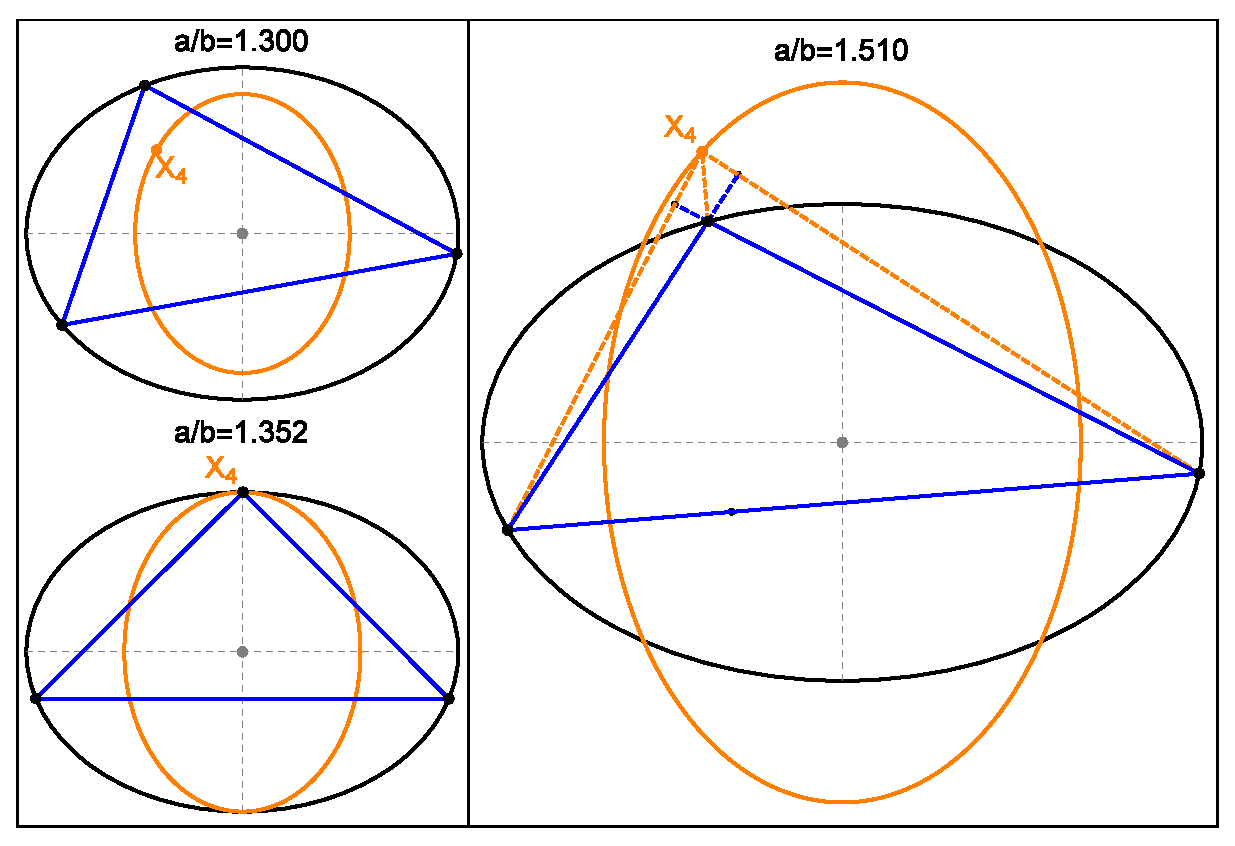
\includegraphics[width=.8\textwidth]{pics/1010_ort_loci.eps}
    \caption{Let
    $\alpha_4=\sqrt{2\,\sqrt {2}-1}\;{\simeq}\;1.352$
    and $H$ be the elliptic locus of $X_4$ (orange), similar to a rotated copy of the EB (black). \textbf{Top Left}: $a/b<\alpha_4$, $H$ is interior to the EB and all 3-periodics (blue) are acute. \textbf{Bot Left}: at $a/b=\alpha_4$, $H$ is tangent to the top and bottom vertices of the EB. The 3-periodic shown is a right triangle since one vertex is at the upper EB vertex where $X_4$ currently is. \textbf{Right}: at $a/b>\alpha_4$, the 3-periodic family will contain both acute and obtuse 3-periodics, corresponding to $X_4$ interior (resp. exterior) to the EB. For any obtuse 3-periodic, $X_4$ will lie within the wedge between sides incident upon the obtuse angle and exterior to the 3-periodic, i.e., exterior to the EB. For the particular aspect ratio shown ($a/b=1.51$), $H$ is identical to a $90^{\circ}$-rotated copy of the EB.}
    \label{fig:orthocenter_loci}
\end{figure}



\subsection{Can a locus be non-smooth?}
\label{sec:orthic-incenter}
Loci considered thus far have been smooth, regular curves.

\begin{proposition}
If $a/b>\alpha_4$ the locus of the Incenter of the 3-periodic's Orthic Triangle comprises four arcs of ellipses, connected at four corners.
\end{proposition}

To see this, let $T$ be a triangle, $T_h$ its Orthic\footnote{Its vertices are the feet of the altitudes.}, and $I_h$ be the latter's Incenter. It is well-known that if $T$ is acute $I_h$ coincides with $T$'s Orthocenter $X_4$. However, for obtuse $T$:

\begin{lemma}
$T_h$ has two vertices outside of $T$, and $I_h$ is ``pinned'' to the obtuse vertex
\label{lem:pinned}
\end{lemma}

This is a known result  \cite[Chapter 1]{coxeter67}, which we revisit in Appendix~\ref{app:orthic-incenter}. This curious phenomenon is illustrated in Figure~\ref{fig:orthic-incenter}. 

\begin{figure}
    \centering
    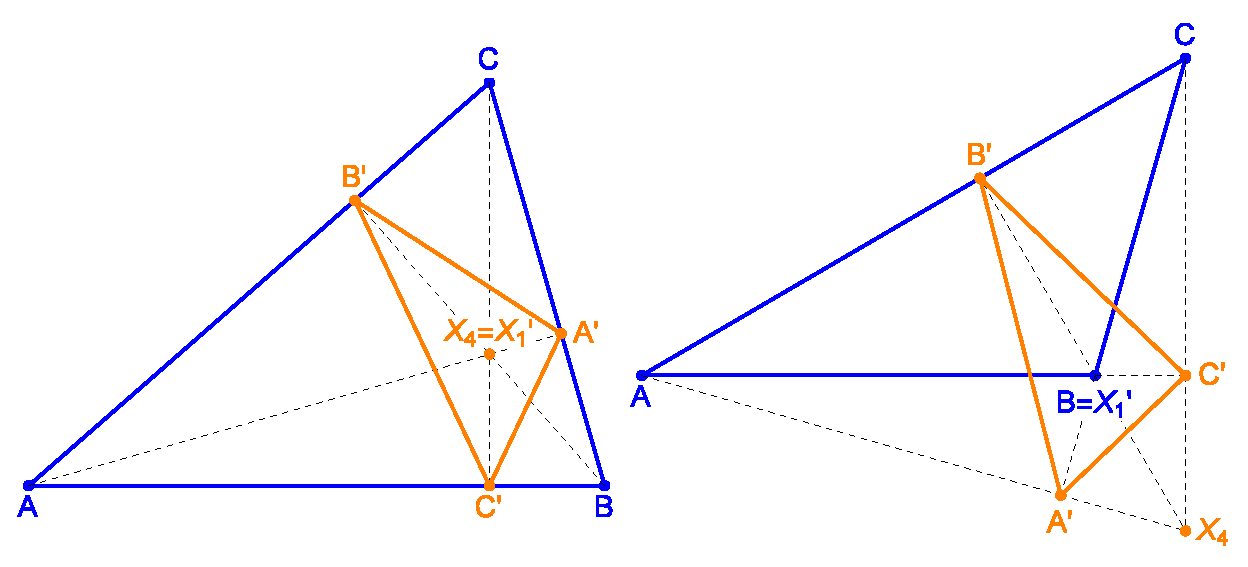
\includegraphics[width=.8\textwidth]{pics/1020_orthic_incenter.eps}
    \caption{\textbf{Left}: If $T=ABC$ is acute (blue), its Orthic $T'=A'B'C'$ is the so-called Fagnano Triangle \cite{rozikov2018-billiards}, whose properties include: (i) inscribed triangle of minimum perimeter, (ii) a 3-periodic of $T$, i.e., the altitudes of $T$ are bisectors of $T'$, i.e., the Orthic Incenter $X_1'$ coincides with the Orthocenter $X_4$. \textbf{Right}: If $T$ is obtuse, two of the Orthic's vertices lie outside $T$, and $X_4$ is exterior to $T$. $T'$ is the Orthic of {\em both} $T$ and {\em acute} triangle $T_e=A{X_4}C$. So the Orthic is the latter's Fagnano Triangle, i.e., $B$ is where both altitudes and bisectors meet. The result is that if $T$ is obtuse at $B$, the Incenter $X_1'$ of the Orthic is $B$. \textbf{Video}: \cite[PL\#06]{reznik2020-playlist-intriguing}}
    \label{fig:orthic-incenter}
\end{figure}

Assume $a/b>\alpha_4$. Since the 3-periodic family contains both acute and obtuse triangles, the locus of $I_h$ transition between acute and obtuse regimes:

\begin{center}
\small
\begin{tabular}{r|c|l}
 3-periodic & $X_4$ wrt EB & $I_h$ location \\ 
 \hline
 acute & interior & Orthocenter $X_4$ \\  
 right triangle & on it & right-angle vertex \\
obtuse & external (3-periodic Excenter) & obtuse vertex, on EB 
%\caption{Incenter behavior acute and obtuse 3-periodics.}
\end{tabular}

\end{center}

In turn, this yields a locus for $I_h$ consisting of four elliptic arcs connected by their endpoints in four corners, Figure~\ref{fig:orthic_incenter_locus}. Notice top and bottom (resp. left and right) arcs belong to the EB (resp. $X_4$ locus).

\begin{figure}
    \centering
    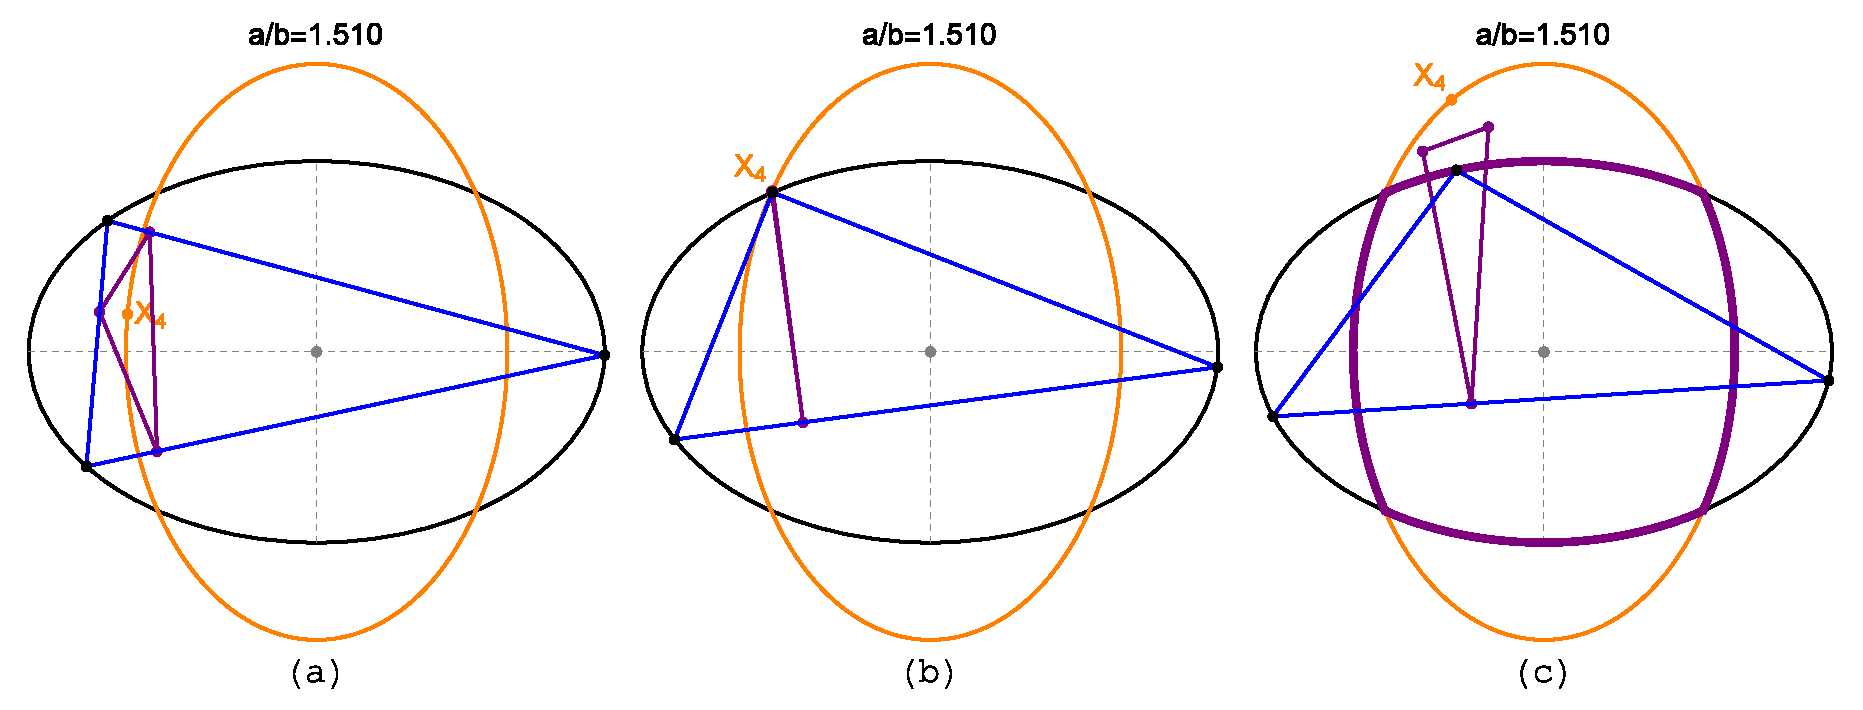
\includegraphics[width=\textwidth]{pics/1030_ort_loci_kink.eps}
    \caption{An $a/b>\alpha_4$ EB is shown (black). Let $T$ and $T_h$ be the 3-periodic and its Orthic Triangle (blue and purple, respectively). \textbf{(a)} $T$ is acute ($X_4$ is interior to the EB), and $I_h=X_4$. \textbf{(b)} $X_4$ is on the EB and $T$ is a right triangle. $T_h$ degenerates to a segment. \textbf{(c)} $X_4$ is exterior to the EB. Two of $T_h$'s vertices are outside $T$. $I_h$ is pinned to $T$'s obtuse vertex, on the EB. $X_4$ is an Excenter of the 3-periodic. The complete locus of $I_h$ comprises therefore 4 elliptic arcs (thick purple) duck-taped at the corners. \textbf{Video}: \cite[PL\#07]{reznik2020-playlist-intriguing}}
    \label{fig:orthic_incenter_locus}
\end{figure}

For the next proposition, 
let $\alpha_h^2$ (resp.~$1/\alpha_h'^2$) be the real root above 1 (resp.~less than 1) of the polynomial $1 + 12 x - 122 x^2 - 52 x^3 + 97 x^4$. Numerically, $\alpha_h{\simeq}1.174$ and $\alpha_h'{\simeq}2.605$.

%\textcolor{red}{ronaldo da pra trocar o $a_1$ %e $b_1$ (usados para os eixos do locus do %incentro) abaixo por talvez u,v ou outra %notacao?}

% TO INSERT: $a/b=\alpha_h''{\simeq}1.982$ the orthic is equilateral.

\begin{proposition}
At $a/b=\alpha_h$ (resp.~$a/b=\alpha_h'$), at the sideways (resp.~upright) 3-periodic, the Orthic is a right triangle, Figure~\ref{fig:right-orthic}. If $a/b>\alpha_h$ some Orthics are obtuse (a family always contains acutes).
\end{proposition}

\begin{proof}
The orthic of an isosceles triangle with vertices $A=(a,0),$ $B=(-u,v)$ and $C=(-u,-v)$ is the isosceles triangle with vertices:
\begin{align*}
A'=&(-u,0)\\
B'=&\left(\frac{-u(a+u)^2+v^2(2a+u) }{(a+u)^2+v^2},\frac{ v( (a+u)^2-v^2)}{(a+u)^2+v^2)}\right)\\
C'=&\left(\frac{-u(a+u)^2+v^2(2a+u) }{(a+u)^2+v^2},- \frac{v( (a+u)^2-v^2)}{(a+u)^2+v^2}\right)
\end{align*}
%
It is rectangle, if and only if, $\langle B'-A',C' -A'\rangle=0$. This condition is expressed by
$r(a,u,v)=(a+u)^2-v(2a+2u+v)=0.$

Using explicit expression to the 3-periodic vertices \cite{garcia2019-incenter}, obtain that  
$u= u(a,b)=a (\delta- {b}^{2})/({a}^{2}-{b}^{2})$ and $v=v(a,b)={b}^{2}\sqrt {2\delta-{a}^{2}-{b}^{2} 
}/({a}^{2}-{b}^{2}).
$
So it follows that $r(a,u,\simeq)=r(a,b)=97a^8-52a^6b^2-122a^4b^4+12a^2b^6+b^8=0.$
The same argument can be applied to the isosceles 3-periodic with vertices:
%
\begin{equation*}
    A=(0,b),\;\;B=(-v(b,a),-u(b,a)),\;\;C=(v(b,a),-u(b,a))
\end{equation*}
%
\noindent The associated orthic triangle will be rectangle, if and only if, $r(b,a)=0$.
\end{proof}


The obtuseness of 3-periodic Orthics is a complex phenomenon with several regimes depending on $a/b$, beyond the scope of this paper. It is explored in  \cite[PL\#08]{reznik2020-playlist-intriguing}.

%Figure~\ref{fig:orthic-orthic} provides experimental details. 

%\begin{figure}
%    \centering
%    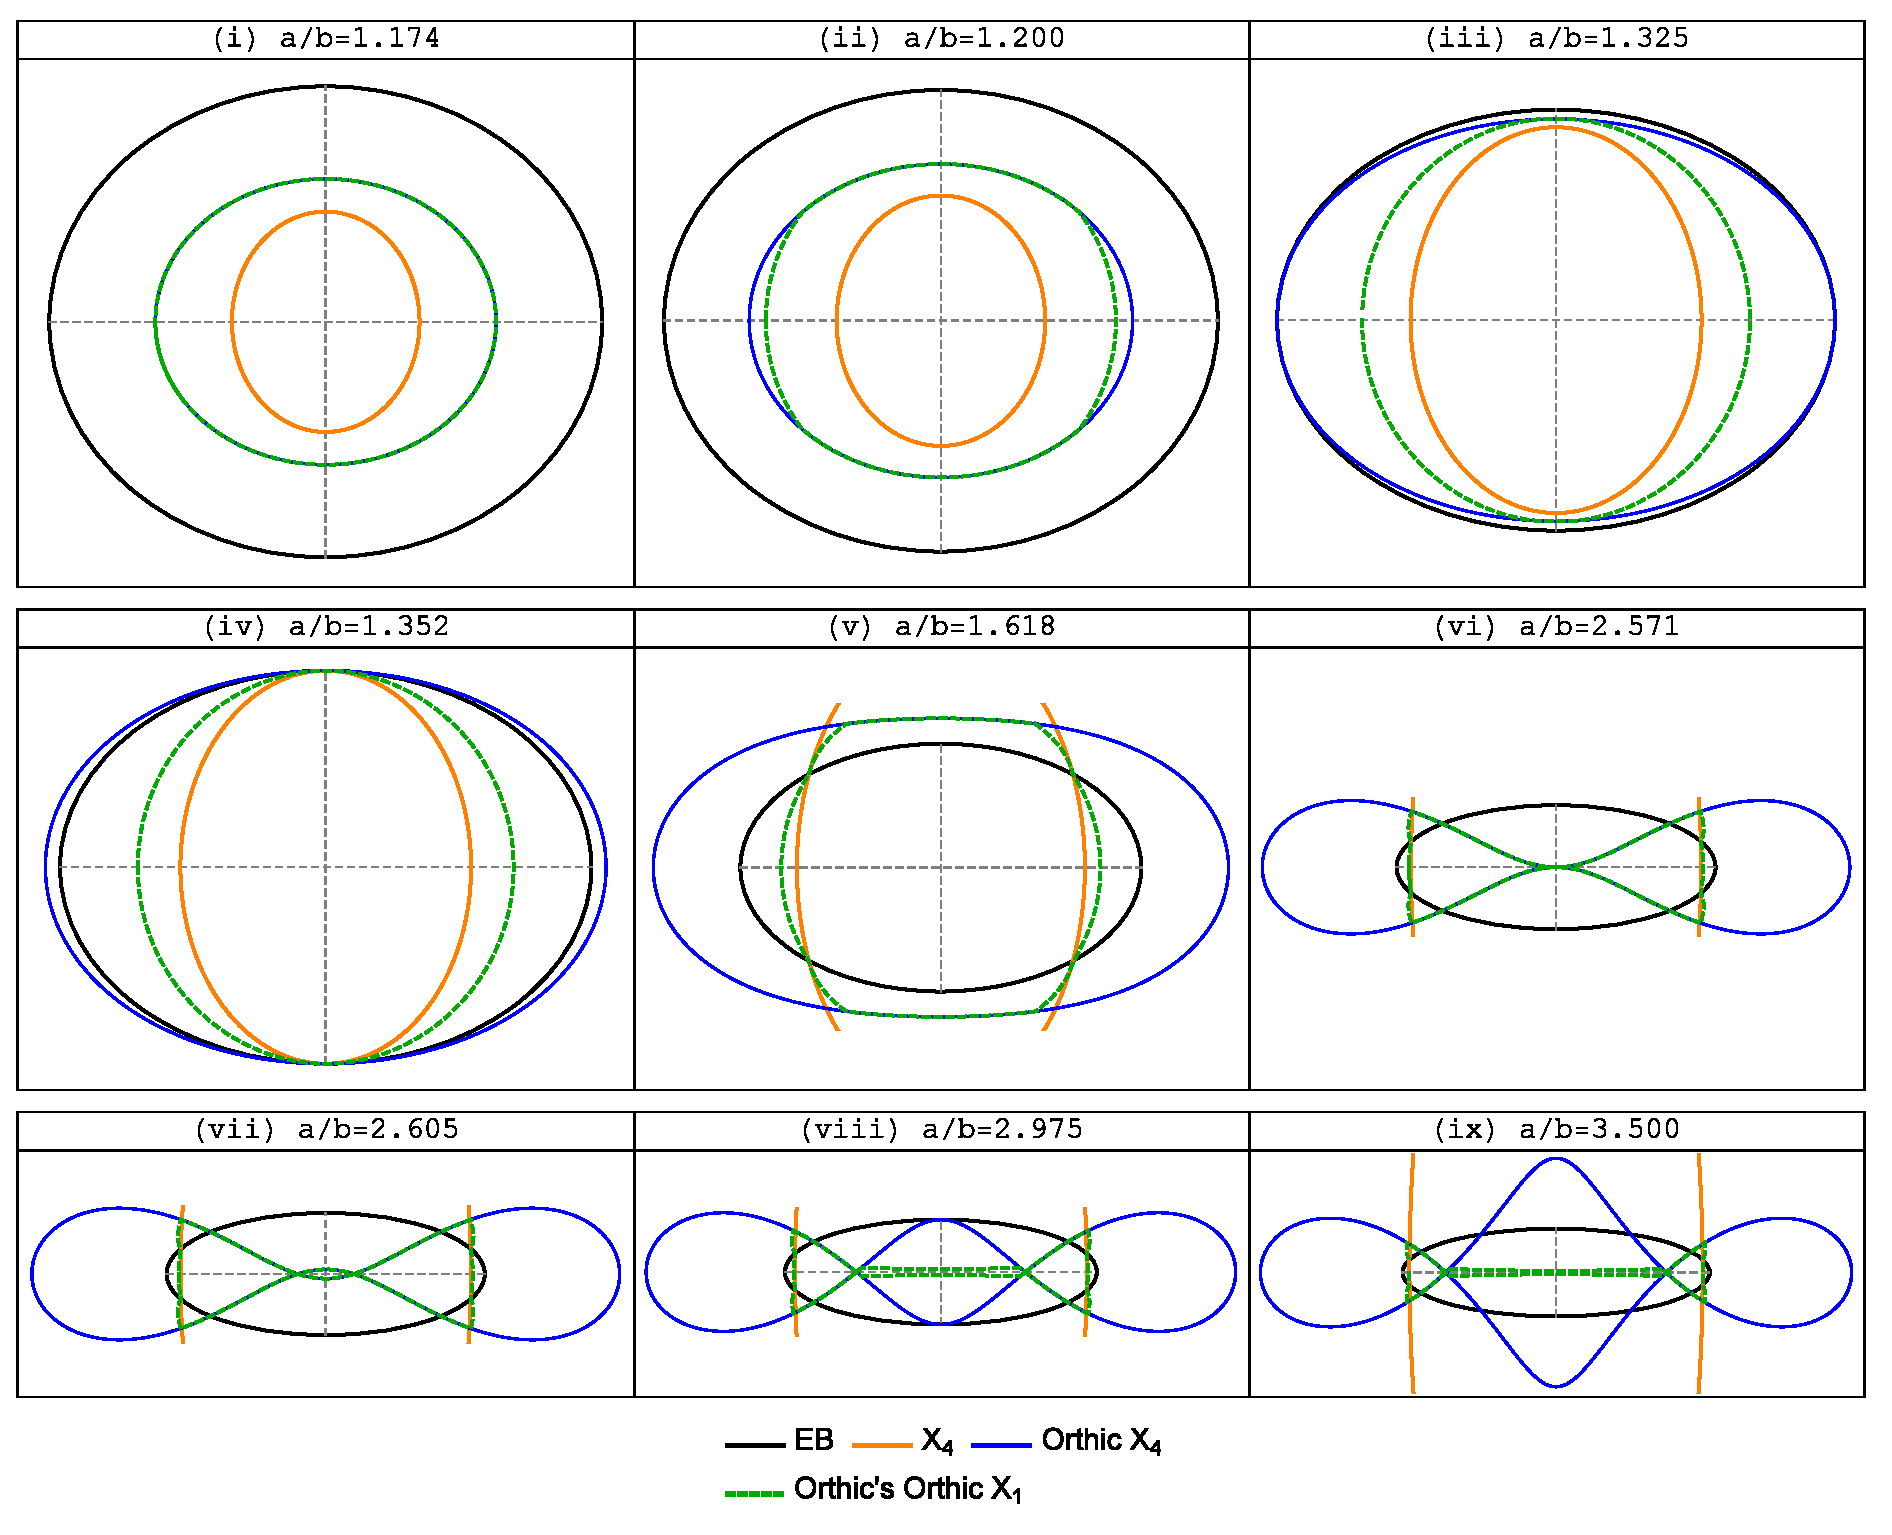
\includegraphics[width=.9\linewidth]{1085_pics_orthic_orthic.eps}
%    \caption{When are Orthics Obtuse? As before, this requires the Orthic Orthic's Incenter $X_1''$ (dashed green) to be detached from the Orthic's Orthocenter $X_4'$ (blue). Let $V$ (resp. $H$) denote either one of the two upright (resp. sideways) isosceles 3-periodics. Notable transitions occur at: (i) $a/b=\alpha_h{\simeq}1.174$, the locus of $X_1''$ is identical to that of $X_4'$, and at $H$, its Orthic is a right-triangle, Figure~\ref{fig:right-orthic} (left); (ii) $a/b>\alpha_h$, one can see $X_1''$ detaching from $X_4'$ indicating a region of obtuse Orthics about the $H$; (iii) At $a/b{\simeq}1.325$ the locus of $X_4'$ touches the EB's left and right vertices at the $H$; (iv) At $a/b=\alpha_4{\simeq}1.352$, the loci of $X_4$ of $X_4'$, and $X_1''$ touch the EB's top and bottom vertices, indicating $V$ are right-triangles and all Orthics not stemming from these are obtuse; (v) At $a/b>\alpha_4$, $X_1''$ tracks $X_4'$ about $V$, indicating some Orthics are acute; (vi) At $a/b{\simeq}2.571$, $X_4'$ two acute Orthics pass through the origin. Above this threshold, the locus of $X_4'$ becomes self-intersecting on the horizontal axis of the EB; (vii) At $a/b=\alpha_h'{\simeq}2.605$, $V$ yield right-triangle Orthics, Figure~\ref{fig:right-orthic} (right). Just above this threshold a new region of obtuse Orthics flares up about $V$; (viii) at $a/b{\simeq}2.965$ $X_4'$ of two obtuse Orthics touch top and bottom vertex of the EB at $V$; (ix) as $a/b$ increases, Orthics about $V$ become more and more obtuse (judging from the deviation between blue and dashed green curves), however two sideway regions of acute Orthic remain where $X_1''$ tracks $X_4'$: these are squeezed to the left and right of the self-intersections of $X_4'$ and the locus of $X_4$. \textbf{Video}: \cite[PL\#08]{reznik2020-playlist-intriguing}}
%    \label{fig:orthic-orthic}
%\end{figure}

\begin{figure}
    \centering
    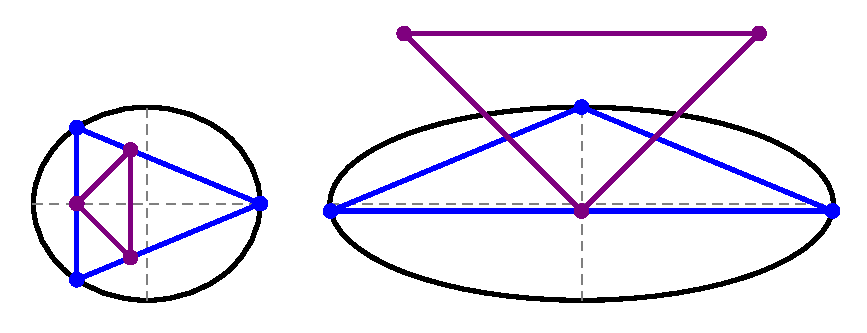
\includegraphics[width=.6\textwidth]{pics/1040_orthic_right_triangle}
    \caption{\textbf{Left}: At $a/b=\alpha_h{\simeq}1.174$, a sideways 3-periodic (blue) has a right-triangle Orthic (purple). If $a/b>\alpha_h$ some Orthics in the family are obtuse. \textbf{Right}: At $a/b=\alpha_h'{\simeq}2.605$, when the 3-periodic is an upright isosceles (obtuse since $a/b>\alpha_h$), its extraverted Orthic is also a right triangle.}
    \label{fig:right-orthic}
\end{figure}

\subsection{Can a Locus be Self-Intersecting?}
\label{sec:x59}
%
%\noindent
%\epigraph{The trees are in their autumn beauty,\\
%The woodland paths are dry,\\
%Under the October twilight the water\\
%Mirrors a still sky;\\
%Upon the brimming water among the stones\\
%Are nine-and-fifty swans.}{\textit{W.B. Yeats}}

Consider a curious TC: $X_{59}$, the ``Isogonal Conjugate of $X_{11}$'' \cite{etc}, i.e., the two centers have reciprocal trilinears.

Experimentally, $X_{59}$ is a continuous curve internally tangent to the EB at its four vertices, and with four self-intersections, Figure~\ref{fig:x59-center}, and as an animation \cite[PL\#12]{reznik2020-playlist-intriguing}. It intersects a line parallel to and infinitesimally away from either axis on six points, so its degree must be at least 6. Producing analytic expressions for salient aspects of its geometry has proven a tough nut to crack, namely, the following are unsolved:

\begin{itemize}
\item What is the degree of its implicit equation?
\item What is $t$ in $P_1(t)=\left(a\cos(t),b\sin(t)\right)$ such that $X_{59}$ is on one of the four self-intersections? For example, at $a/b=1.3$ (resp. $1.5$), $t$, given in degrees is ${\simeq}32.52^\circ$ (resp. $29.09^\circ$), Figure~\ref{fig:x59-center} (left-bottom).
\item What is $a/b$ such that if $X_{59}$ is on one of the lower self-intersection on the $y$-axis, the 3-periodic is a right triangle? Numerically, this occurs when $a/b=\alpha_{59}^\perp\,{\simeq}\,1.58$ and $t{\simeq}27.92^\circ$, Figure~\ref{fig:x59-center} (right).
\end{itemize}

\begin{figure}
    \centering
    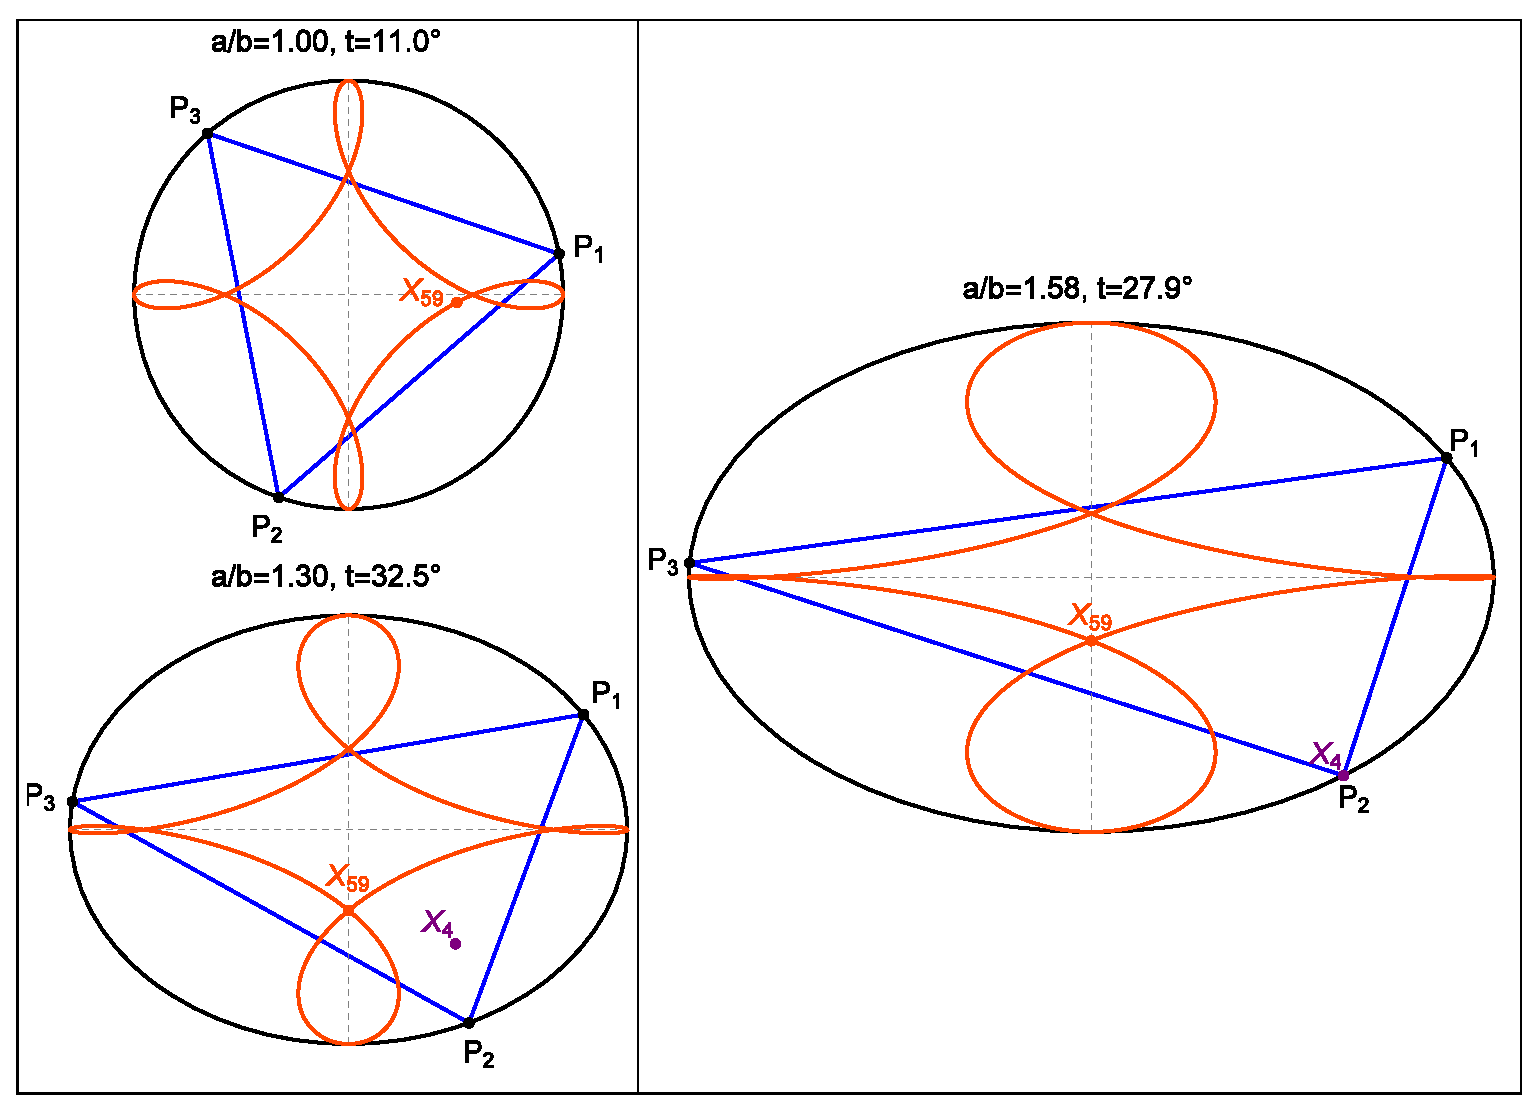
\includegraphics[width=.8\textwidth]{pics/1050_x59_center.eps}
    \caption{The locus of $X_{59}$ is a continuous curve with four self-intersections, and at least a sextic. It is tangent to the EB at its four vertices. \textbf{Top Left}: circular EB, $X_{59}$ is symmetric about either axis. \textbf{Bottom Left}: $a/b=1.3$, at $t{\simeq}32.5^\circ$ $X_{59}$ is at the lower self-intersection and the 3-periodic is acute ($X_4$ is interior). \textbf{Right}: at $a/b=\alpha_{59}^\perp\,{\simeq}\,1.58$ the following feat is possible: $X_{59}$ is at the lower self-intersection {\em and} the 3-periodic is a right-triangle ($X_4$ is on $P_2$). This occurs at $t{\simeq}27.9^\circ$. \textbf{Video}: \cite[PL\#12]{reznik2020-playlist-intriguing}}
    \label{fig:x59-center}
\end{figure}

\subsection{Can a Locus be Non-compact}
\label{sec:x26}
$X_{26}$ is the Circumcenter of the Tangential Triangle \cite{mw}. Its sides are tangent to the Circumcircle at the vertices. If the 3-periodic is a right-triangle, its hypotenuse is a diameter of the Circumcircle, and $X_{26}$ is unbounded.

We saw above that:

\begin{itemize}
\item $a/b<\alpha_4$, the 3-periodic family is all-acute, i.e., the locus of $X_{26}$ is compact. Figure~\ref{fig:orthocenter_loci} (top left).
\item $a/b=\alpha_4$, the family is all-acute except when one of its vertices coincides with the top or bottom vertex of the EB, Figure~\ref{fig:orthocenter_loci} (bottom left). In this case the 3-periodic is a right triangle and $X_{26}$ is unbounded.
\item $a/b>\alpha_4$, the family features both acute and obtuse triangles. The transition occurs at for four right-angle 3-periodics whose $X_4$ is on the EB, Figure~\ref{fig:orthic_incenter_locus}(b). Here too $X_{26}$ flies off to infinity, Figure~\ref{fig:x26}.
\end{itemize}

\begin{figure}
    \centering
    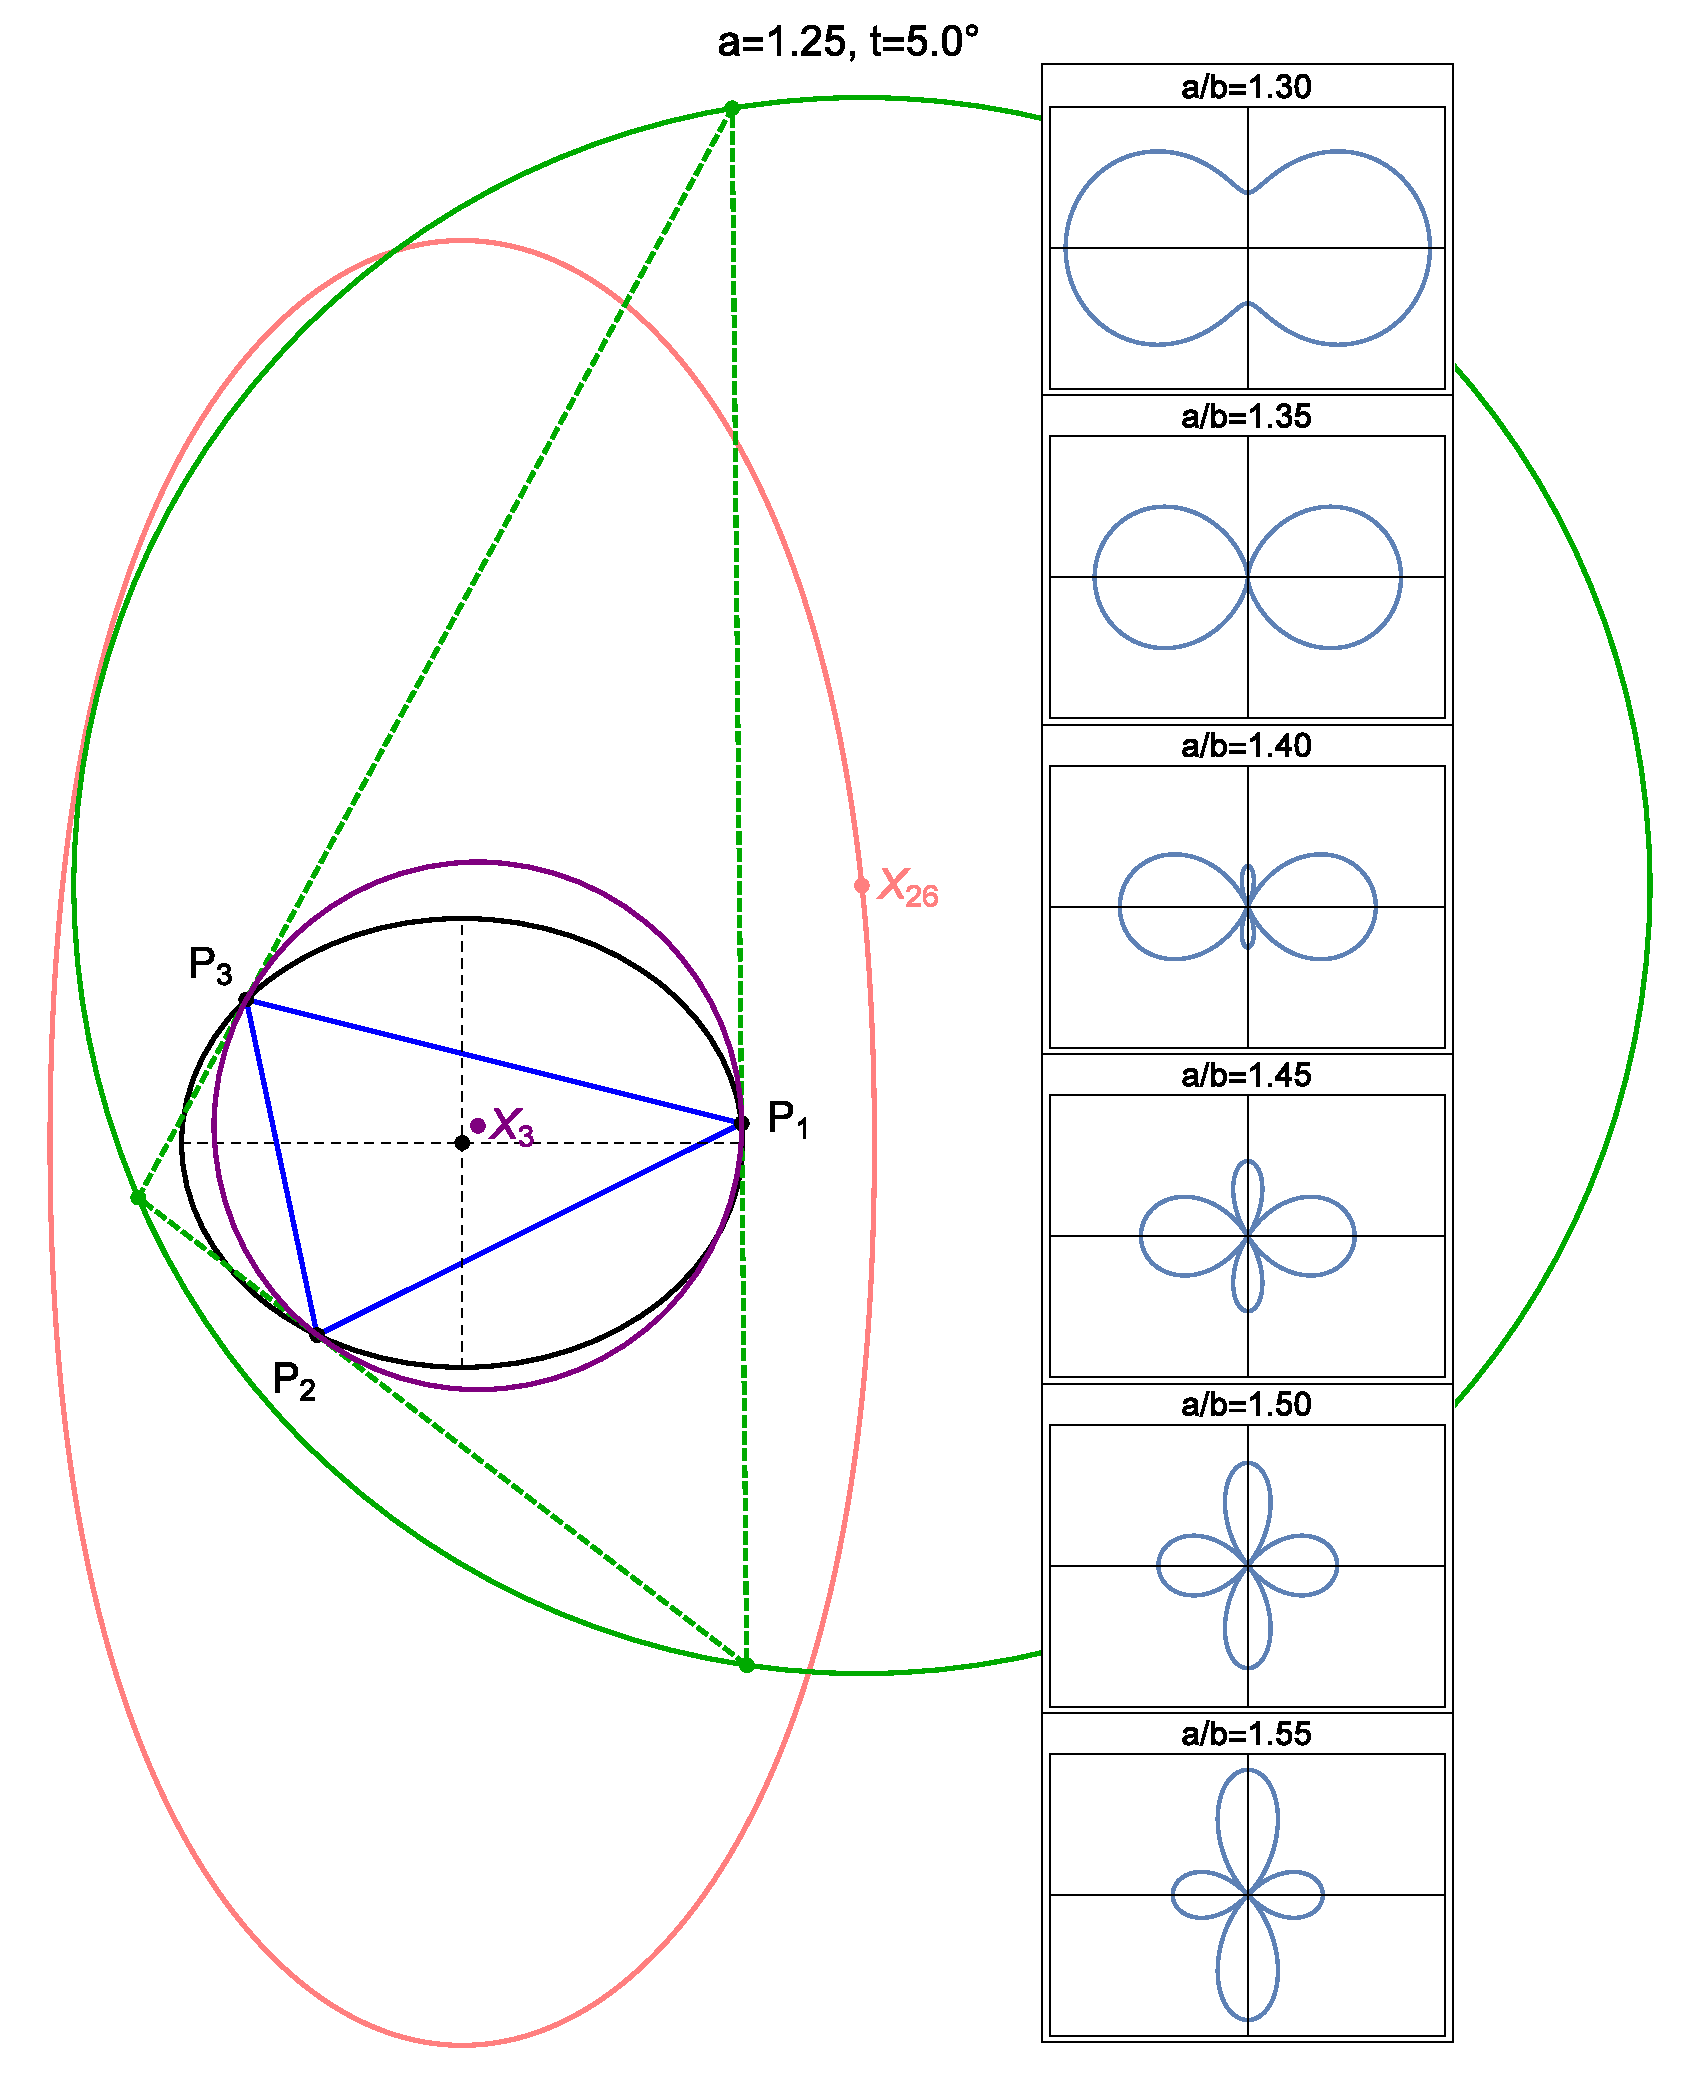
\includegraphics[width=.8\textwidth]{pics/1060_x26.eps}
    \caption{The locus of $X_{26}$ for a 3-periodic (blue) in an $a/b=1.25$ EB (black). Also shown is the 3-periodic's Circumcircle (purple) and its Tangential Triangle \cite{mw} (dashed green). $X_{26}$ is the center of the latter's Circumcircle (solid green). Its locus is non-elliptic. In fact, when $a/b{\geq}\alpha_4$, the 3-periodic family will contain right-triangles ($X_4$ crosses the EB). At these events, $X_{26}$ flies off to infinity. The right inset shows an inversion of $X_{26}$  with respect to the EB center for various values of $a/b$. When $a/b>\alpha_4$, the inversion goes through the origin, i.e., $X_{26}$ is at infinity.}
    \label{fig:x26}
\end{figure}

